\documentclass[a0paper,12pt]{article}
\usepackage[landscape,top=5cm,bottom=3cm,right=5cm,left=5cm]{geometry}
\usepackage{graphicx}
\usepackage[T1]{fontenc}
\usepackage{lmodern}
\usepackage{tikz}
\usepackage{color}
\usepackage{multicol}
\usepackage{moresize}

\newenvironment{Figure}
  {\par\medskip\noindent\minipage{\linewidth}}
  {\endminipage\par\medskip}

\tikzset{
  every overlay node/.style={
    draw=black,fill=white,rounded corners,anchor=north west,
  },
}
% Usage:
% \tikzoverlay at (-1cm,-5cm) {content};
% or
% \tikzoverlay[text width=5cm] at (-1cm,-5cm) {content};
\def\tikzoverlay{%
   \tikz[baseline,overlay]\node[draw=white,every overlay node]
}%

\begin{document}

\begin{tikzpicture}[remember picture,overlay] 
    \node[opacity=1.0] (background) at (current page.center) {
    
\includegraphics[width=\paperwidth,height=\paperheight]{./background.jpg}
};
\end{tikzpicture}

%%% here goes the title and all
%\tikzoverlay[draw=white,text width=\textwidth] at (10cm,-4cm) {
%    \fontsize{4cm}{1em}\selectfont Modelling Memory Across Scale
%};
%

\begin{minipage}{\textwidth}
    \centering
    \fontsize{4cm}{1em}\selectfont \textcolor{red}{Modelling Memory Across Scale}
    \\
    \fontsize{1.5cm}{1em}\selectfont Aditya Gilra, Aviral Goel, Dilawar Singh,
    Harsha Rani, Sahil Moza, Subhasis Ray, Upinder Bhalla
\end{minipage}


%% Three columns
\vspace{5cm}
\setlength{\columnsep}{6cm}
\begin{multicols}{3}
%% Introduction here.
    \section*{\HUGE \textcolor{red}{Introduction}}
\HUGE

\begin{Figure}
\begin{itemize}
    \item Modeling across scale, bottom-up. A single neuron, 
\end{itemize}

    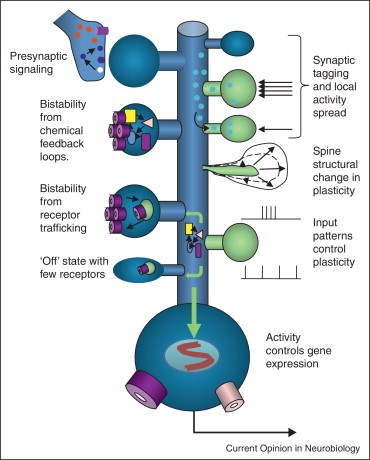
\includegraphics[width=0.5\textwidth]{./images/computation_inside_neurons.jpg}
\end{Figure}

\end{multicols}

\end{document}
